\documentclass[10pt,a4paper]{article}
\usepackage[utf8]{inputenc}
\usepackage[T1]{fontenc}
\usepackage{mathptmx}
\usepackage[margin=2.2cm]{geometry}
\usepackage{amsmath,booktabs,graphicx,microtype,caption,titlesec,enumitem}
\usepackage[hidelinks]{hyperref}
\captionsetup{font=small,labelfont=bf}
\titlespacing*{\section}{0pt}{9pt}{3pt}
\titlespacing*{\subsection}{0pt}{6pt}{2pt}
\setlist{nosep,leftmargin=1.4em}
\setlength{\parskip}{3pt}\setlength{\parindent}{0pt}
\newcommand{\unit}[1]{\,\mathrm{#1}}
\title{\vspace{-1.2cm}\Large\bfseries Evidence-Aware Benchmarking of Biochar-Assisted Anaerobic Digestion Kinetics: Reproducibility, Dose-Response Validation and Forecasting Baselines}
\author{Nikan Haghighatjue\\ \small MSc Chemical Engineering, Sapienza Universit\`a di Roma\\ \small \url{https://github.com/thisisnikan/Biochar-AD-Kinetics}}
\date{\small Technical research report accompanying software version 0.1.0 (release candidate), 16 November 2026.\\ Not peer reviewed.}
\begin{document}
\maketitle
\vspace{-0.6cm}
\section*{Abstract}
Biochar is widely reported to improve methane production in anaerobic digestion (AD), but the published evidence is difficult to compare and kinetic models are usually judged by goodness of fit. This report asks three bounded questions of three public datasets, using held-out prediction error only. (i) On 10 food-waste batch reactors from Koz\l{}owski et al.\ (2025), the modified Gompertz curve has the lowest leave-one-reactor-out error in all four treatments (5.8 to 12.8 mL CH$_4$ g$^{-1}$ VS). (ii) On five published biochar doses from Valentin and Bia\l{}owiec (2024), the project's own log-quadratic dose-response hypothesis is not supported: a log-linear form predicts a held-out dose with 11.1\% error in methane potential against 31.6\%. (iii) On 100 retrospective cycles from 27 bottles in the dataset of Sanglier et al.\ (2022), a three-point recent-rate extrapolation forecasts end-of-cycle methane from a 12.5-day prefix with 8.4\% error against 13.7\% for the best kinetic model; the kinetic models are better only from a 6.5-day prefix. All three results were regenerated from committed inputs for this report. The datasets answer different questions and are not pooled. None of the results establishes a mechanism, a causal biochar effect, cross-study prediction or an operational digital twin. Two of the three results count against the more complex model.

\section{Motivation and research questions}
Reported effects of biochar on AD vary with substrate, inoculum, biochar feedstock, pyrolysis temperature, dose and reporting convention. Raw reactor trajectories and inoculum blanks are often unavailable, so models are fitted to treatment means and compared by $R^2$. A curve that fits well can still predict poorly, and a flexible dose-response term can be fitted to almost any small table. The project therefore fixes the evaluation rule before looking at the answer: every comparison uses error on reactors, doses or time points that the model has not seen, and every dataset is restricted to the question its design can support.

\begin{enumerate}
\item[\textbf{Q1}] Which standard cumulative-methane curve best predicts an unseen replicate reactor?
\item[\textbf{Q2}] Does a curved (log-quadratic) dose response predict an unseen biochar dose better than simpler forms?
\item[\textbf{Q3}] Given the first part of a batch cycle, do kinetic models forecast the end-of-cycle yield better than baselines that use no kinetic model?
\end{enumerate}

\section{Dataset provenance and eligibility}
Table~\ref{tab:data} lists the evidence. Source files are identified by SHA-256 hashes recorded in the repository, and each derived table is rebuilt by a committed script that checks the hash first.

\begin{table}[h]\centering\small
\caption{Datasets, their role and the limits on their use. All are third-party data under their own licences.}\label{tab:data}
\begin{tabular}{@{}p{2.9cm}p{4.6cm}p{2.1cm}p{5.6cm}@{}}\toprule
Source & Content used & Evidence type & Limits \\ \midrule
Koz\l{}owski et al.\ (2025), CC BY 4.0 & 12 reactor trajectories and 3 inoculum blanks, food waste, 37\,$^\circ$C, 21 d, 5 g L$^{-1}$ carbon material; 505 readings per reactor & Independent experiment, reactor level & 10 reactors eligible (two excluded as in the source workbook); 2 or 3 reactors per treatment; one dose, one temperature \\
Valentin and Bia\l{}owiec (2024), CC BY 4.0 & Published kinetic parameters at 0, 2, 4, 6, 8 g L$^{-1}$ wheat-straw biochar, glucose, 37\,$^\circ$C & Independent experiment, table level & Five points, no replicate spread, no raw trajectories; doses up to 8 g L$^{-1}$ only \\
Sanglier et al.\ (2022), Etalab 2.0 & 8,403 methane records from 363 bottle/batch cycles, two laboratories & Retrospective benchmark & Methane units asserted, not source-verified; intervention metadata incomplete; not admitted as external validation \\
Synthetic curves & Generated by the package & Software demonstration & No scientific evidence \\ \bottomrule
\end{tabular}\end{table}

Two Koz\l{}owski reactors are marked ineligible, following the authors' own workbook: one torrefaction replicate recorded no methane and one pyrolysis replicate ended about 16\% below its siblings. They remain in the dataset, and Section~\ref{sec:limits} reports the result with them included. For the Sanglier forecasting benchmark, a cycle is eligible if it was recorded for at least 13 days and carries no technical-fault flag, which gives 100 cycles from 27 bottles (15 and 12 per laboratory) with final times from 13.7 to 34.6 days (median 20.8). A separate, pre-registered admission review of the same dataset concluded that it cannot externally validate any model in the repository; that decision is unchanged here.

\section{Models and evaluation protocols}
\textbf{Curves (Q1, Q3).} For cumulative methane $M(t)$ with potential $P$, maximum rate $R$, lag $\lambda$ and rate constant $k$:
\begin{align*}
\text{first order:}\quad & M = P\,(1-e^{-kt}), \\
\text{modified Gompertz:}\quad & M = P\exp\{-\exp[(eR/P)(\lambda-t)+1]\}, \\
\text{logistic:}\quad & M = P\,/\,\{1+\exp[(4R/P)(\lambda-t)+2]\}, \\
\text{two-pool first order:}\quad & M = P_f(1-e^{-k t}) + P_s(1-e^{-\rho k t}),\quad 0<\rho<1 .
\end{align*}
The Gompertz reparameterisation is that of Zwietering et al.\ (1990). Parameters are estimated by bounded nonlinear least squares.

\textbf{Q1 protocol.} Within each treatment one shared curve is fitted to all reactors but one and scored on the complete trajectory of the held-out reactor. The score is the mean root-mean-square error (RMSE) over held-out reactors, in mL CH$_4$ g$^{-1}$ VS. A reactor is never split between training and test. Information criteria are reported but not used for ranking, because points within a cumulative trajectory are autocorrelated.

\textbf{Q2 protocol.} With $x=\ln(1+d)$ for dose $d$ in g L$^{-1}$, three forms are fitted by ordinary least squares to the logarithm of each published parameter $\theta\in\{P,R\}$: constant ($\ln\theta=a$), log-linear ($a+bx$) and log-quadratic ($a+bx+cx^2$). The log-quadratic form is the project's hypothesis, since it permits an optimum dose. Each dose is held out in turn and predicted from the other four. Each dose is a single table row, so no replicate of the held-out dose can enter training.

\textbf{Q3 protocol.} For prefixes of 6.5, 9.5 and 12.5 days each method predicts the final recorded yield of the cycle. Persistence holds the last reading. The recent-rate baseline fits a straight line to the last three prefix readings, clips a negative slope to zero and extrapolates. Kinetic models are fitted to the prefix only. The score is the absolute relative endpoint error, averaged within each bottle and then across bottles so that every bottle has equal weight. Because the error is relative, the unresolved methane unit does not enter it. Uncertainty is a paired bootstrap of whole bottles within laboratory (5,000 draws, fixed seed).

\textbf{Checks applied to all three.} Blank-correction sensitivity (five alternative corrections of the Koz\l{}owski yields); parameter identifiability (correlation and conditioning of the fitted parameters, and the share of fits that stop at a bound); and exact regeneration of every committed output.

\section{Results}
\textbf{Q1.} Modified Gompertz ranks first in every treatment (Fig.~\ref{fig:one}a). The logistic curve is second in three treatments and first order in one. The same ranking is obtained under all five blank corrections, which move final yields by at most 1.64\%. With two or three reactors per treatment, no interval can be placed on the RMSE differences; the result is a consistent ranking across four treatments, not a tested difference.

The fitted Gompertz parameters also give within-study effects relative to the food-waste control (delta-method 95\% intervals on the log response ratio). Methane potential is higher with all three materials: hydrochar $+8.4\%$ [3.9, 13.2], pyrolysis biochar $+4.5\%$ [0.1, 9.0], torrefied material $+11.9\%$ [7.1, 16.8]. Maximum rate is lower or unchanged: $-2.4\%$ [$-6.7$, 2.1], $-7.4\%$ [$-11.2$, $-3.5$] and $-1.6\%$ [$-5.5$, 2.4]. The biochar and torrefaction arms have two eligible reactors, the three effects share one control (correlations 0.86 to 0.99), and the intervals exclude blank-correction and fit uncertainty. These are descriptive within-study contrasts.

\begin{figure}[h]\centering
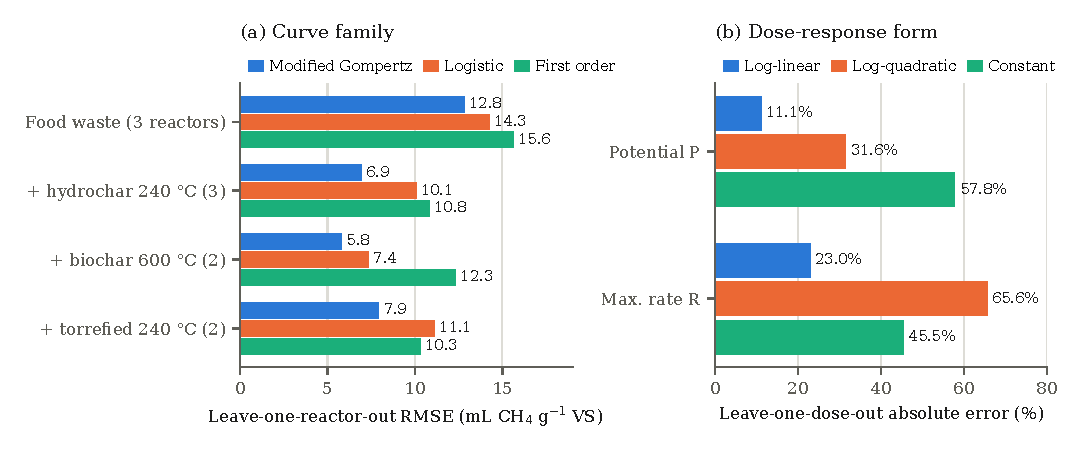
\includegraphics[width=\linewidth]{figures/fig1_model_selection.pdf}
\caption{Held-out error. (a) Leave-one-reactor-out RMSE by curve family and treatment, Koz\l{}owski et al.\ (2025); eligible reactors in brackets. (b) Leave-one-dose-out mean absolute percentage error by dose-response form, Valentin and Bia\l{}owiec (2024), five doses. Drawn from \texttt{results/experimental/} and \texttt{results/external-dose/}.}\label{fig:one}
\end{figure}

\textbf{Q2.} The log-linear form has the lowest held-out error for both parameters (Fig.~\ref{fig:one}b): for $P$, RMSE 46.6 against 75.8 mL CH$_4$ g$^{-1}$ VS for the log-quadratic form and 138.4 for the constant; for $R$, 14.6 against 33.1 and 27.3 mL CH$_4$ g$^{-1}$ VS d$^{-1}$. For the rate, the log-quadratic form is worse than assuming no dose effect at all. The hypothesis is therefore rejected as tested on this table.

\textbf{Q3.} Table~\ref{tab:fc} and Fig.~\ref{fig:two} show that the answer depends on the prefix. From 6.5 days the two-pool model is clearly better than the recent-rate baseline (difference $-32.0$ points, interval $-43.3$ to $-21.2$). From 9.5 days the two are indistinguishable ($+0.2$, $-5.4$ to $+5.2$). From 12.5 days the baseline is better ($+5.3$, $+2.5$ to $+7.3$), and the same holds when two failing control bottles are removed (8.4\% against 13.6\%, 88 cycles, 25 bottles).

\begin{table}[h]\centering\small
\caption{Equal-bottle mean absolute relative endpoint error (\%), 100 cycles from 27 bottles, Sanglier et al.\ (2022).}\label{tab:fc}
\begin{tabular}{@{}lrrrrr@{}}\toprule
Prefix & Persistence & Recent rate & First order & Mod.\ Gompertz & Two-pool \\ \midrule
6.5 d & 40.7 & 51.0 & 23.1 & 29.7 & \textbf{19.0} \\
9.5 d & 28.5 & \textbf{14.7} & 16.4 & 22.9 & 14.8 \\
12.5 d & 18.6 & \textbf{8.4} & 14.4 & 17.4 & 13.7 \\ \bottomrule
\end{tabular}\end{table}

\begin{figure}[h]\centering
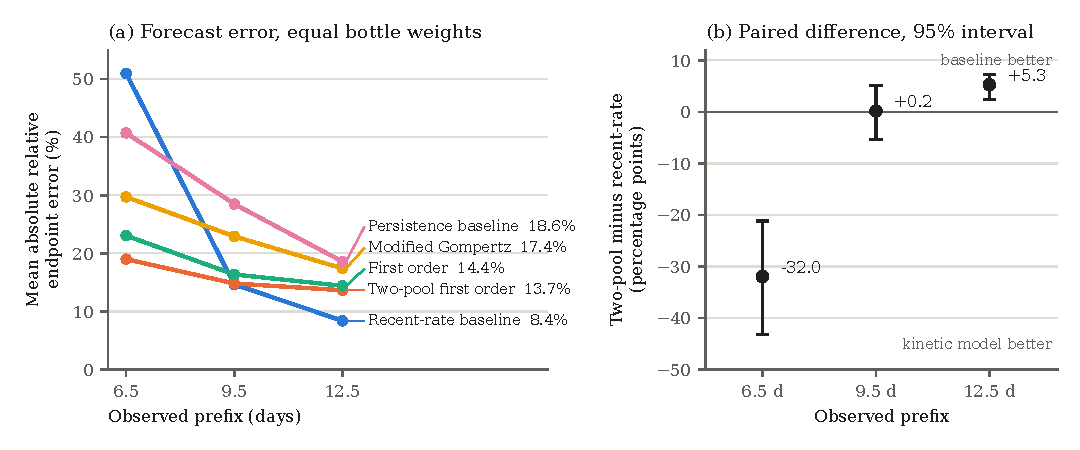
\includegraphics[width=\linewidth]{figures/fig2_forecasting.pdf}
\caption{Forecasting benchmark. (a) Error against observed prefix for five of the seven methods. (b) Paired difference between the two-pool model and the recent-rate baseline with conditional bootstrap 95\% intervals; positive values favour the baseline. Drawn from \texttt{results/forecasting/summary.csv}.}\label{fig:two}
\end{figure}

\section{Interpretation, model failures and limitations}\label{sec:limits}
\textbf{What failed.} (1) The log-quadratic dose response, the central modelling idea of the project, lost to a straight line in $\ln(1+d)$. (2) Kinetic models did not beat a three-point extrapolation once most of the cycle had been observed. (3) The eight-parameter dose and temperature model is not identifiable even on the noise-controlled synthetic demonstration (two parameters correlate at about 0.96), and no real dataset in the repository varies both dose and temperature with replicates. (4) Between 81\% and 96\% of two-pool prefix fits stop at a parameter bound, so their forecast accuracy says nothing about their parameters.

\textbf{Why the negative dose result is weaker than it looks.} With five doses, the log-quadratic form is fitted to four points with three coefficients, so held-out prediction at the end doses is extrapolation with almost no residual freedom. A simulation of the same test shows that a design at the minimum eligibility gate recovers a truly curved response in at most 7 of 24 runs, while a grid extending to 70 g L$^{-1}$ recovers it in 18 to 24 of 24. The present table cannot exclude an optimum at or above 8 g L$^{-1}$. The correct statement is that the available data give no support for curvature, not that curvature is absent.

\textbf{Why the forecasting result is weaker than it looks.} Eligibility requires a long cycle and the target is the last recorded time, both chosen retrospectively. At least a quarter of the cycles end at 13.7 days, which is 1.2 days after the 12.5-day cutoff; over such a short horizon a local linear extrapolation is expected to do well. The bootstrap intervals are conditional on these bottles and laboratories and ignore shared batch effects. The benchmark does not test a fixed prospective horizon or unseen bottles.

\textbf{Excluded reactors.} With all 12 Koz\l{}owski reactors included, modified Gompertz still ranks first in every treatment, but in the two affected treatments the margin nearly vanishes (37.8 against 38.1, and 236.65 against 236.68 mL CH$_4$ g$^{-1}$ VS), because the error is then dominated by the aberrant reactor and not by curve shape.

\textbf{Numerical reproducibility.} The curve-family, dose-response, forecasting and blank-sensitivity outputs regenerate byte for byte. The upstream prefix-fit audit does not: on a different machine 53 of 1,500 fits differ, the largest by 0.24 in relative error, all in weakly identified fits. Re-running the benchmark from the regenerated fits changes one tabulated value (two-pool at 6.5 days, 19.0\% to 18.9\%) and no conclusion.

\textbf{What is not claimed.} No direct interspecies electron transfer or other mechanism; no causal methane enhancement beyond the descriptive within-study contrasts; no pooled accuracy across the three datasets; no cross-study generalisation; no external validation by the Sanglier data; no operational digital twin.

\section{Reproducibility}
\begin{verbatim}
git clone https://github.com/thisisnikan/Biochar-AD-Kinetics && cd Biochar-AD-Kinetics
python -m venv .venv && source .venv/bin/activate && pip install -e ".[dev]"
ruff check . && pytest -q                          # 300 tests
biochar-ad benchmark-experimental --output results/experimental      # Q1
biochar-ad benchmark-external-dose --output results/external-dose    # Q2
python scripts/benchmark_sanglier_forecasts.py                       # Q3
python scripts/analyze_kozlowski_blank_sensitivity.py
python scripts/make_report_figures.py                                # Figs 1 and 2
\end{verbatim}
The suite passed on Python 3.10, 3.12 and 3.13 (pandas 2.3, 3.0 and 3.1). The commands must be run from a clone, because the datasets are not packaged with the wheel. The full audit record is \texttt{docs/REPRODUCTION\_AUDIT\_2026\_11.md}.

\section{Conclusions and experimental requirements}
On the evidence available, the modified Gompertz curve is the best of three standard curves for predicting an unseen replicate; a monotone log-linear dose response is preferred to a curved one over 0 to 8 g L$^{-1}$; and a kinetic model earns its place in forecasting only early in a cycle. Each statement is limited to one dataset.

The next step is experimental, not computational. The frozen Stage~A protocol in the repository requires, at one digestion temperature: a zero-dose substrate control; at least three amended doses of one characterised biochar, with a dose range extending well beyond the expected optimum; at least three replicate reactors per dose (the variance analysis in the repository indicates four); inoculum blanks; individual reactor trajectories of 14 to 20 days or longer; and recorded inoculum-to-substrate ratio, dose basis and biochar properties. The decision rule (select the simplest form unless a more complex one lowers whole-dose held-out RMSE by more than 10\%) was fixed before any such data exist. A forecasting claim additionally needs a horizon, cutoff and method fixed before a new batch is measured.

\section*{Statement on tools}
Code development and the reproduction audit were carried out with an AI coding assistant (Claude, Anthropic). No measurement in this report was generated by a model; all values are computed from the cited public datasets.

\section*{References}
\small
\begin{enumerate}[label={[\arabic*]},leftmargin=2em]
\item Koz\l{}owski, M., Papaj, B., Sobieraj, K., \'Swiechowski, K., Kosiorowska, K., Bia\l{}owiec, A. (2025). The effect of different carbon materials' addition on the biomethane production from food waste. \emph{Scientific Reports} 15, 18728. \url{https://doi.org/10.1038/s41598-025-02564-0}
\item Valentin, M. T., Bia\l{}owiec, A. (2024). Impact of using glucose as a sole carbon source to analyze the effect of biochar on the kinetics of biomethane production. \emph{Scientific Reports} 14, 8656. \url{https://doi.org/10.1038/s41598-024-59313-y}
\item Sanglier, M., Leurent, A., Moscoviz, R., Rouez, M., Battimelli, A., Escudi\'e, R., Guilayn, F. (2022). Supplementation of biochar and trace elements to increase the resilience of food waste anaerobic digestion: a long-term study [dataset]. Recherche Data Gouv. \url{https://doi.org/10.57745/BUJORT}
\item Zwietering, M. H., Jongenburger, I., Rombouts, F. M., van 't Riet, K. (1990). Modeling of the bacterial growth curve. \emph{Applied and Environmental Microbiology} 56(6), 1875--1881. \url{https://doi.org/10.1128/aem.56.6.1875-1881.1990}
\end{enumerate}
\end{document}
